\chapter{Outcome and Result}

% TODO: rewrite to independent from the test plan (may removed)
\section{Simulation Result}
\begin{figure}[h]
    \centering
    
\includegraphics[width=1\linewidth]{figures/6.1.png}
    \caption{\centering{Simulation result of \textbf{a.} Seed with incorrect parameters and \textbf{b.} Seed with normal parameters}}
    \label{fig:6.1}
\end{figure}
To validate the functionality and ensure the reliability of the pulse channel module, a controlled randomized regression test was designed and implemented. This test serves as a comprehensive evaluation of the module’s performance across several critical aspects. Specifically, it examines the module's ability to execute memory read and write operations efficiently, preserve data accuracy during these processes, and manage potential errors effectively. These assessments are crucial for identifying and resolving any latent issues that could compromise the module's functionality in practical applications. The results of this testing process provide significant insights into the module's behavior and confirm its expected performance. \autoref{fig:6.1} illustrates two simulation outcomes, both generated using Intel ModelSim, which visually validate the module’s operation under the given test scenarios.

% A key component of this test is the use of a seed value to manage the randomization process. This seed, which begins at one and increments sequentially by one with each iteration, introduces controlled variability into the test inputs. The randomization ensures that the module's memories are subjected to diverse data patterns. These values are simultaneously applied to the module's memory system and a corresponding software model, which serves as a theoretical benchmark. By comparing the module's output with the software model, the hardware's accuracy is rigorously verified.

% \autoref{table:error_results} offers an illustrative snapshot of the first ten iterations of the regression test, outlining several key performance metrics. The column labeled "Seed" denotes the specific randomization seed used during each test, providing insight into the exact conditions under which the test was conducted. The "Time" metric indicates the elapsed duration from when a pulse is triggered to when the corresponding error is detected. Additionally, the "Error/Delta" value represents the ratio between the observed error and the reference delta, offering a quantitative measure of performance discrepancies. It is calculated by
% \begin{equation}
% \frac{Error}{Delta} = \frac{|\text{theoretical value} - \text{actual value}|}{|\text{current hardware output} - \text{previous hardware output}|}
% \end{equation}
% Finally, the "Pulse Number" specifies the sequential order of the pulse that produced the largest error-to-delta ratio during that iteration. Together, these detailed metrics enable us to thoroughly assess how the module responds under a wide spectrum of conditions, ultimately affirming its reliability and adherence to our stringent performance criteria.

% \begin{table}[h]
% \centering
% \caption{Simulation results for first 10 seeds}
% \begin{tabular}{|c|c|c|c|}
% \hline
% Seed & Time (ns) & Error/Delta & Pulse Number \\
% \hline
% 1 & 159490 & 0.0035 & 3 \\
% 2 & 175960 & 0.1932 & 4 \\
% 3 & 189310 & 0.0096 & 5 \\
% 4 & 156640 & 0.0149 & 2 \\
% 5 & 159900 & 0.0022 & 2 \\
% 6 & 159090 & 0.3055 & 3 \\
% 7 & 161220 & 0.2224 & 3 \\
% 8 & 163910 & 0.1640 & 3 \\
% 9 & 134220 & 0.0164 & 0 \\
% 10 & 134220 & 0.0302 & 0 \\
% \hline
% \end{tabular}
% \label{table:error_results}
% \end{table}


\section{Board Result}
The system is examined using Xilinx's Integrated Logic Analyzer (ILA) to validate signals from multiple modules, including the single pulse channel module.  
\begin{figure}[h]
    \centering
    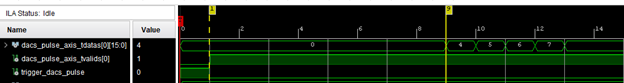
\includegraphics[width=1\linewidth]{figures/ila.png}
    \caption{ILA monitored the result from the top level.}
    \label{fig:ila}
\end{figure}
% The ILA plays a crucial role in verifying the precise timing of waveform generation triggered externally. Traditional oscilloscopes often struggle to capture such high-resolution timing details, making the ILA essential for this role. 
A 55-sample waveform, starting from a nonzero value at 50 ns, is transmitted to the hardware and captured by the ILA (see \autoref{fig:ila}). The first output appears after 8 cycles, with each cycle lasting 10 nanoseconds. This timing results in an 80-nanosecond delay, confirming that the pulse generation operates well within the sub-microsecond range required for quantum control hardware. Furthermore, the ILA data shows that data updates occur every 10 nanoseconds, demonstrating the rapid switching performance essential for high-speed applications. Additionally, an external oscilloscope recorded a pulse sequence in \autoref{fig:osc}, further verifying the overall functionality and behavior of the design.
\begin{figure}[h]
    \centering
    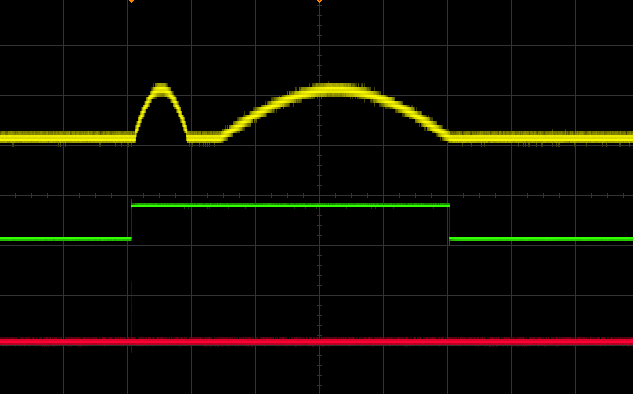
\includegraphics[width=.85\linewidth]{figures/one_trig_seq.png}
    \caption{\centering{A single pulse sequence captured on an oscilloscope. The yellow line is the pulse sequence, the green line is the valid signal, and the red line is the trigger signal.}}
    \label{fig:osc}
\end{figure}
% The ILA plays a 

\section{Resource Utilization}

In FPGA design, efficient resource utilization is essential for ensuring a high-quality, reliable system. One of the most critical aspects of this evaluation is timing analysis. After implementation, the Xilinx Vivado tool generates an in-depth timing report that details the minimum and maximum delay paths within the design. Generated reports in \autoref{fig:sta} confirm that the critical timing parameters—both setup and hold times—meet the specified constraints.
\begin{figure}[ht]
    \centering
    
\includegraphics[width=1\linewidth]{figures/timimg_report.png}
    \caption{Partial timing report from Vivado on the worst slack (top) and hold (bottom).}
    \label{fig:sta}
\end{figure}
This timing verification is crucial because it ensures that all synchronous elements operate correctly within the designated clock cycle, preventing data corruption and operational failures. 

\autoref{table:chip_utilization} shows that only a small fraction of the FPGA resources are used. This low usage proves the design's efficiency. Minimal resource usage reduces power consumption. It also helps the FPGA maintain optimal timing and routing. This efficiency is ideal for scalable systems that may need future modifications. It validates the careful design decisions made during synthesis and optimization.

\begin{table}[ht]
\centering
\begin{tabular}{|l|r|r|r|r|}
\hline
On-Chip & Power (W) & Used & Available & Utilization (\%) \\ \hline
Clocks                  & 0.034   & 3     & ---    & ---      \\ \hline
CLB Logic               & 0.018   & 30403 & ---    & ---      \\ \hline
\quad LUT as Logic      & 0.015   & 12671 & 274080 & 4.62     \\ \hline
\quad CARRY8            & 0.002   & 909   & 34260  & 2.65     \\ \hline
\quad Register          & $<$0.001& 12952 & 548160 & 2.36     \\ \hline
\quad LUT as Shift Register & $<$0.001 & 4   & 144000 & $<$0.01 \\ \hline
\quad Others            & 0.000   & 567   & ---    & ---      \\ \hline
Signals                 & 0.029   & 24867 & ---    & ---      \\ \hline
Block RAM               & 0.174   & 128   & 912    & 14.04    \\ \hline
DSPs                    & $<$0.001& 2     & 2520   & 0.08     \\ \hline
I/O                     & 0.014   & 36    & 328    & 10.98    \\ \hline
PS8                     & 2.472   & 1     & ---    & ---      \\ \hline
Static Power            & 0.750   &       &        &          \\ \hline
\quad PS Static         & 0.098   &       &        &          \\ \hline
\quad PL Static         & 0.653   &       &        &          \\ \hline
Total                   & 3.492   &       &        &          \\ \hline
\end{tabular}
\caption{Post-Implementation Resource Utilization Reported by Vivado}
\label{table:chip_utilization}
\end{table}
